% Exam slides (beamer, Sapienza colors). Build with `make slides` or run
% pdflatex twice for the page totals. Figures come straight from ../figures/
% so a recompile after retraining keeps the deck in sync.
\documentclass[aspectratio=169,11pt]{beamer}

\usepackage[T1]{fontenc}
\usepackage[utf8]{inputenc}
\usepackage{helvet}\renewcommand{\familydefault}{\sfdefault}
\usepackage{booktabs}
\usepackage{tikz}
\graphicspath{{../figures/}}

% ── Sapienza palette ────────────────────────────────────────────────────────
\definecolor{sapienzaRed}{RGB}{130,36,51}     % Rosso Sapienza
\definecolor{sapienzaDark}{RGB}{45,41,38}
\definecolor{sapienzaGray}{RGB}{111,111,111}
\definecolor{sapienzaPale}{RGB}{247,244,241}
\definecolor{okGreen}{RGB}{0,99,0}
\definecolor{warnRed}{RGB}{208,59,59}
\definecolor{accBlue}{RGB}{42,120,214}

% ── Minimal custom theme ────────────────────────────────────────────────────
\usetheme{default}
\usefonttheme{professionalfonts}
\setbeamertemplate{navigation symbols}{}
\setbeamercolor{structure}{fg=sapienzaRed}
\setbeamercolor{titlelike}{fg=sapienzaRed}
\setbeamercolor{normal text}{fg=sapienzaDark}
\setbeamercolor{alerted text}{fg=warnRed}
\setbeamercolor{example text}{fg=okGreen}
\setbeamercolor{block title}{bg=sapienzaRed,fg=white}
\setbeamercolor{block body}{bg=sapienzaPale,fg=sapienzaDark}
\setbeamertemplate{itemize item}{\textcolor{sapienzaRed}{\rule[0.45ex]{0.6ex}{0.6ex}}}
\setbeamertemplate{itemize subitem}{\textcolor{sapienzaGray}{\rule[0.45ex]{0.5ex}{0.5ex}}}
\setbeamerfont{frametitle}{size=\large,series=\bfseries}
\setbeamertemplate{frametitle}{%
  \vskip1ex
  {\usebeamerfont{frametitle}\textcolor{sapienzaRed}{\insertframetitle}}%
  \ifx\insertframesubtitle\empty\else
    \\[-0.2ex]{\small\textcolor{sapienzaGray}{\insertframesubtitle}}%
  \fi
  \vskip0.4ex
  {\color{sapienzaRed}\hrule height 1.2pt}
}
\setbeamertemplate{footline}{%
  \leavevmode\hbox{\begin{beamercolorbox}[wd=\paperwidth,ht=2.6ex,dp=1.2ex,leftskip=1em,rightskip=1em]{normal text}
    \tiny\textcolor{sapienzaGray}{True Lethality Engine — Statistical Machine Learning, Sapienza}
    \hfill\tiny\textcolor{sapienzaGray}{\insertsection\quad|\quad\insertframenumber/\inserttotalframenumber}
  \end{beamercolorbox}}%
}

% Part-divider helper: full-red slide announcing presenter + section
\newcommand{\partdivider}[3]{%
  {\setbeamercolor{background canvas}{bg=sapienzaRed}
  \begin{frame}[plain]
    \vfill
    {\color{white}\Huge\bfseries Part #1\\[1ex]}
    {\color{white}\LARGE #2\\[3ex]}
    {\color{white!80!sapienzaRed}\large Presenter: #3}
    \vfill
  \end{frame}}%
}

\newcommand{\srcnote}[1]{{\tiny\textcolor{sapienzaGray}{#1}}}

% ── Metadata ────────────────────────────────────────────────────────────────
\title{\textbf{The True Lethality Engine}\\
  \large Predicting the real danger of D\&D 5e combat from 34{,}907 recorded encounters}
\subtitle{Statistical Machine Learning — Final Project}
\author{%
  Presenter 1 (NOME) \and Presenter 2 (NOME) \and
  Presenter 3 (NOME) \and Presenter 4 (NOME)}
\institute{Sapienza Università di Roma}
\date{A.Y. 2025/2026}

\begin{document}

% ── Title ───────────────────────────────────────────────────────────────────
{\setbeamercolor{background canvas}{bg=sapienzaRed}
\begin{frame}[plain]
  \vfill\centering
  {\color{white!85!sapienzaRed}\small SAPIENZA UNIVERSITÀ DI ROMA — STATISTICAL MACHINE LEARNING\\[3ex]}
  {\color{white}\Huge\bfseries The True Lethality Engine\\[1.2ex]}
  {\color{white}\large Predicting the real danger of D\&D 5e combat\\ from 34{,}907 recorded encounters\\[4ex]}
  {\color{white!80!sapienzaRed}\normalsize Presenter 1 · Presenter 2 · Presenter 3 · Presenter 4\\[1ex]}
  {\color{white!80!sapienzaRed}\small \texttt{dnd-appraising.streamlit.app} \quad · \quad \texttt{github.com/danpinocontrollino/project-dnd}}
  \vfill
\end{frame}}

\begin{frame}{Roadmap}{Four parts, one question: how dangerous is this monster, \emph{really}?}
  \begin{columns}[T]
    \column{0.5\textwidth}
      \textbf{\textcolor{sapienzaRed}{Part 1 — The problem \& the data}}\\
      \small Why the official difficulty system fails; turning 153k chat log lines into a dataset; reading damage out of statblocks.\\[2ex]
      \textbf{\textcolor{sapienzaRed}{Part 2 — Model \& honest evaluation}}\\
      \small Combat-math features; calibrated XGBoost; why we validate by \emph{campaign}; confidence intervals.
    \column{0.5\textwidth}
      \textbf{\textcolor{sapienzaRed}{Part 3 — Guards \& simulation}}\\
      \small Where observational data lies (DM mercy); three domain guards; calibrating one of them with 490k simulated battles.\\[2ex]
      \textbf{\textcolor{sapienzaRed}{Part 4 — Benchmarks \& the product}}\\
      \small The course model zoo; a linear model that wins AUC and still loses; the live app; limits.
  \end{columns}
\end{frame}

% ════════════════════════════════════════════════════════════════════════════
\partdivider{1}{The problem \& the data}{NOME 1}
\section{Part 1 — Problem \& data}

\begin{frame}{D\&D combat in 60 seconds}
  \begin{columns}[T]
    \column{0.55\textwidth}
      \begin{itemize}
        \item A \textbf{party} (3–6 heroes, levels 1–20) fights \textbf{monsters} run by the Dungeon Master.
        \item Every monster has a \textbf{Challenge Rating (CR)}: the official difficulty score, 0–30.
        \item The rulebook (DMG p.82) estimates encounter difficulty: sum monster XP, apply a multiplier for monster count, compare with per-level thresholds.
      \end{itemize}
    \column{0.42\textwidth}
      \begin{block}{The official promise}
        A CR-5 monster $\approx$ a fair fight for four level-5 heroes.
      \end{block}
      \begin{block}{The reality}
        CR is a \emph{design intention}, never validated against play.
      \end{block}
  \end{columns}
\end{frame}

\begin{frame}{Our question is an estimand, not a score}
  \begin{block}{Target}
    $\eta(x) = P(\text{party wins} \mid \text{encounter } x)$, calibrated — then invert it:
    the \textbf{True Lethality Level} is the party level at which a balanced party of 4
    reaches a target win rate (default 65\%), found by binary search on $\eta$.
  \end{block}
  \begin{itemize}
    \item Everything downstream consumes \textbf{probabilities}, so calibration is a first-class requirement, not a nicety.
    \item Boundary verdicts instead of fake precision: \textcolor{okGreen}{\textbf{trivial}} (wins $\geq$ target even at level 1) and \textcolor{warnRed}{\textbf{beyond deadly}} (below target even at level 20).
  \end{itemize}
\end{frame}

\begin{frame}{The data: FIREBALL — real play, not simulation}
  \begin{columns}[T]
    \column{0.55\textwidth}
      \begin{itemize}
        \item 1{,}471 JSONL logs of real Discord games (Avrae bot) — 153{,}829 turn snapshots.
        \item Outcome inferred from terminal HP states; unresolved fights dropped.
        \item \textbf{34{,}907 resolved encounters} across \textbf{1{,}462 campaigns}.
        \item Party win base rate: \textbf{83.0\%} — remember this number.
      \end{itemize}
    \column{0.43\textwidth}
      \begin{block}{Encounter-level row}
        party level/size/roles $\times$ monster roster aggregates $\times$ outcome
      \end{block}
      \srcnote{parse\_fireball.py — count-weighted means, apex maxima, pooled sums; party levels clipped to 1–20, rosters to 30}
  \end{columns}
\end{frame}

\begin{frame}{The Attack Potency problem}{The bestiary has HP and AC — but nothing about how hard a monster hits}
  \begin{itemize}
    \item Solution: \textbf{parse offense from the statblock text itself} (SRD JSON):
          \texttt{+9 to hit}, \texttt{12 (2d6+5)}, ``makes \emph{three} attacks'', \texttt{DC 14}, spell lists.
    \item Per-action segmentation separates \textbf{sustained DPR} (weapon routine) from \textbf{burst} (breath weapon, best spell — Lich: DPR 45, burst 100 via \emph{Power Word Kill}).
    \item Coverage: \textbf{321/762} monsters from real statblocks; the rest imputed from the DMG's design table by CR.
  \end{itemize}
  \begin{exampleblock}{Bugs this catches}
    Pooled regexes over-counted: versatile weapons (``7 \ldots{} \emph{or} 8 two-handed'') summed both ($\to$ 24 monsters overstated); dragon breath leaked into multiattack math (Adult Red DPR 72.6 $\to$ 58, true $\approx$ 45–48).
  \end{exampleblock}
\end{frame}

\begin{frame}{Playing fair with the rulebook}{If we claim to beat the DMG, we must implement the DMG correctly}
  \begin{columns}[T]
    \column{0.52\textwidth}
      \begin{itemize}
        \item The app's ``by the book'' column runs the \textbf{real DMG p.82 math}: total XP $\times$ count multiplier $\to$ equivalent single-monster CR (inverse XP table).
        \item $6 \times$ CR-1 monsters $= 1{,}200$ XP $\times\, 2 = 2{,}400 \approx$ \textbf{one CR-6 monster} — not ``CR 1''.
      \end{itemize}
    \column{0.46\textwidth}
      \begin{block}{Why it matters}
        Reported discrepancies measure our model against the rulebook's \emph{best effort} — not against a strawman.
      \end{block}
      \srcnote{official\_encounter\_estimate() — 9 regression tests incl.\ the DMG's own worked example}
  \end{columns}
\end{frame}

% ════════════════════════════════════════════════════════════════════════════
\partdivider{2}{Model \& honest evaluation}{NOME 2}
\section{Part 2 — Model \& evaluation}

\begin{frame}{Feature engineering: put the combat math in the features}
  \begin{columns}[T]
    \column{0.55\textwidth}
      \small
      \begin{itemize}
        \item \textbf{To-hit geometry}: party hit chance vs monster AC; monster hit chance vs estimated party AC (both from the actual d20 rule).
        \item \textbf{The damage race}: rounds-to-kill on both sides; \texttt{lethality\_log\_ratio}.
        \item \textbf{Nova pressure}: \texttt{burst\_vs\_pc\_hp} — can one action delete a hero?
        \item Trait $\times$ composition interactions (magic resistance $\times$ arcane party, \ldots).
        \item DMG XP budget with the count multiplier — the rulebook as a feature.
      \end{itemize}
    \column{0.43\textwidth}
      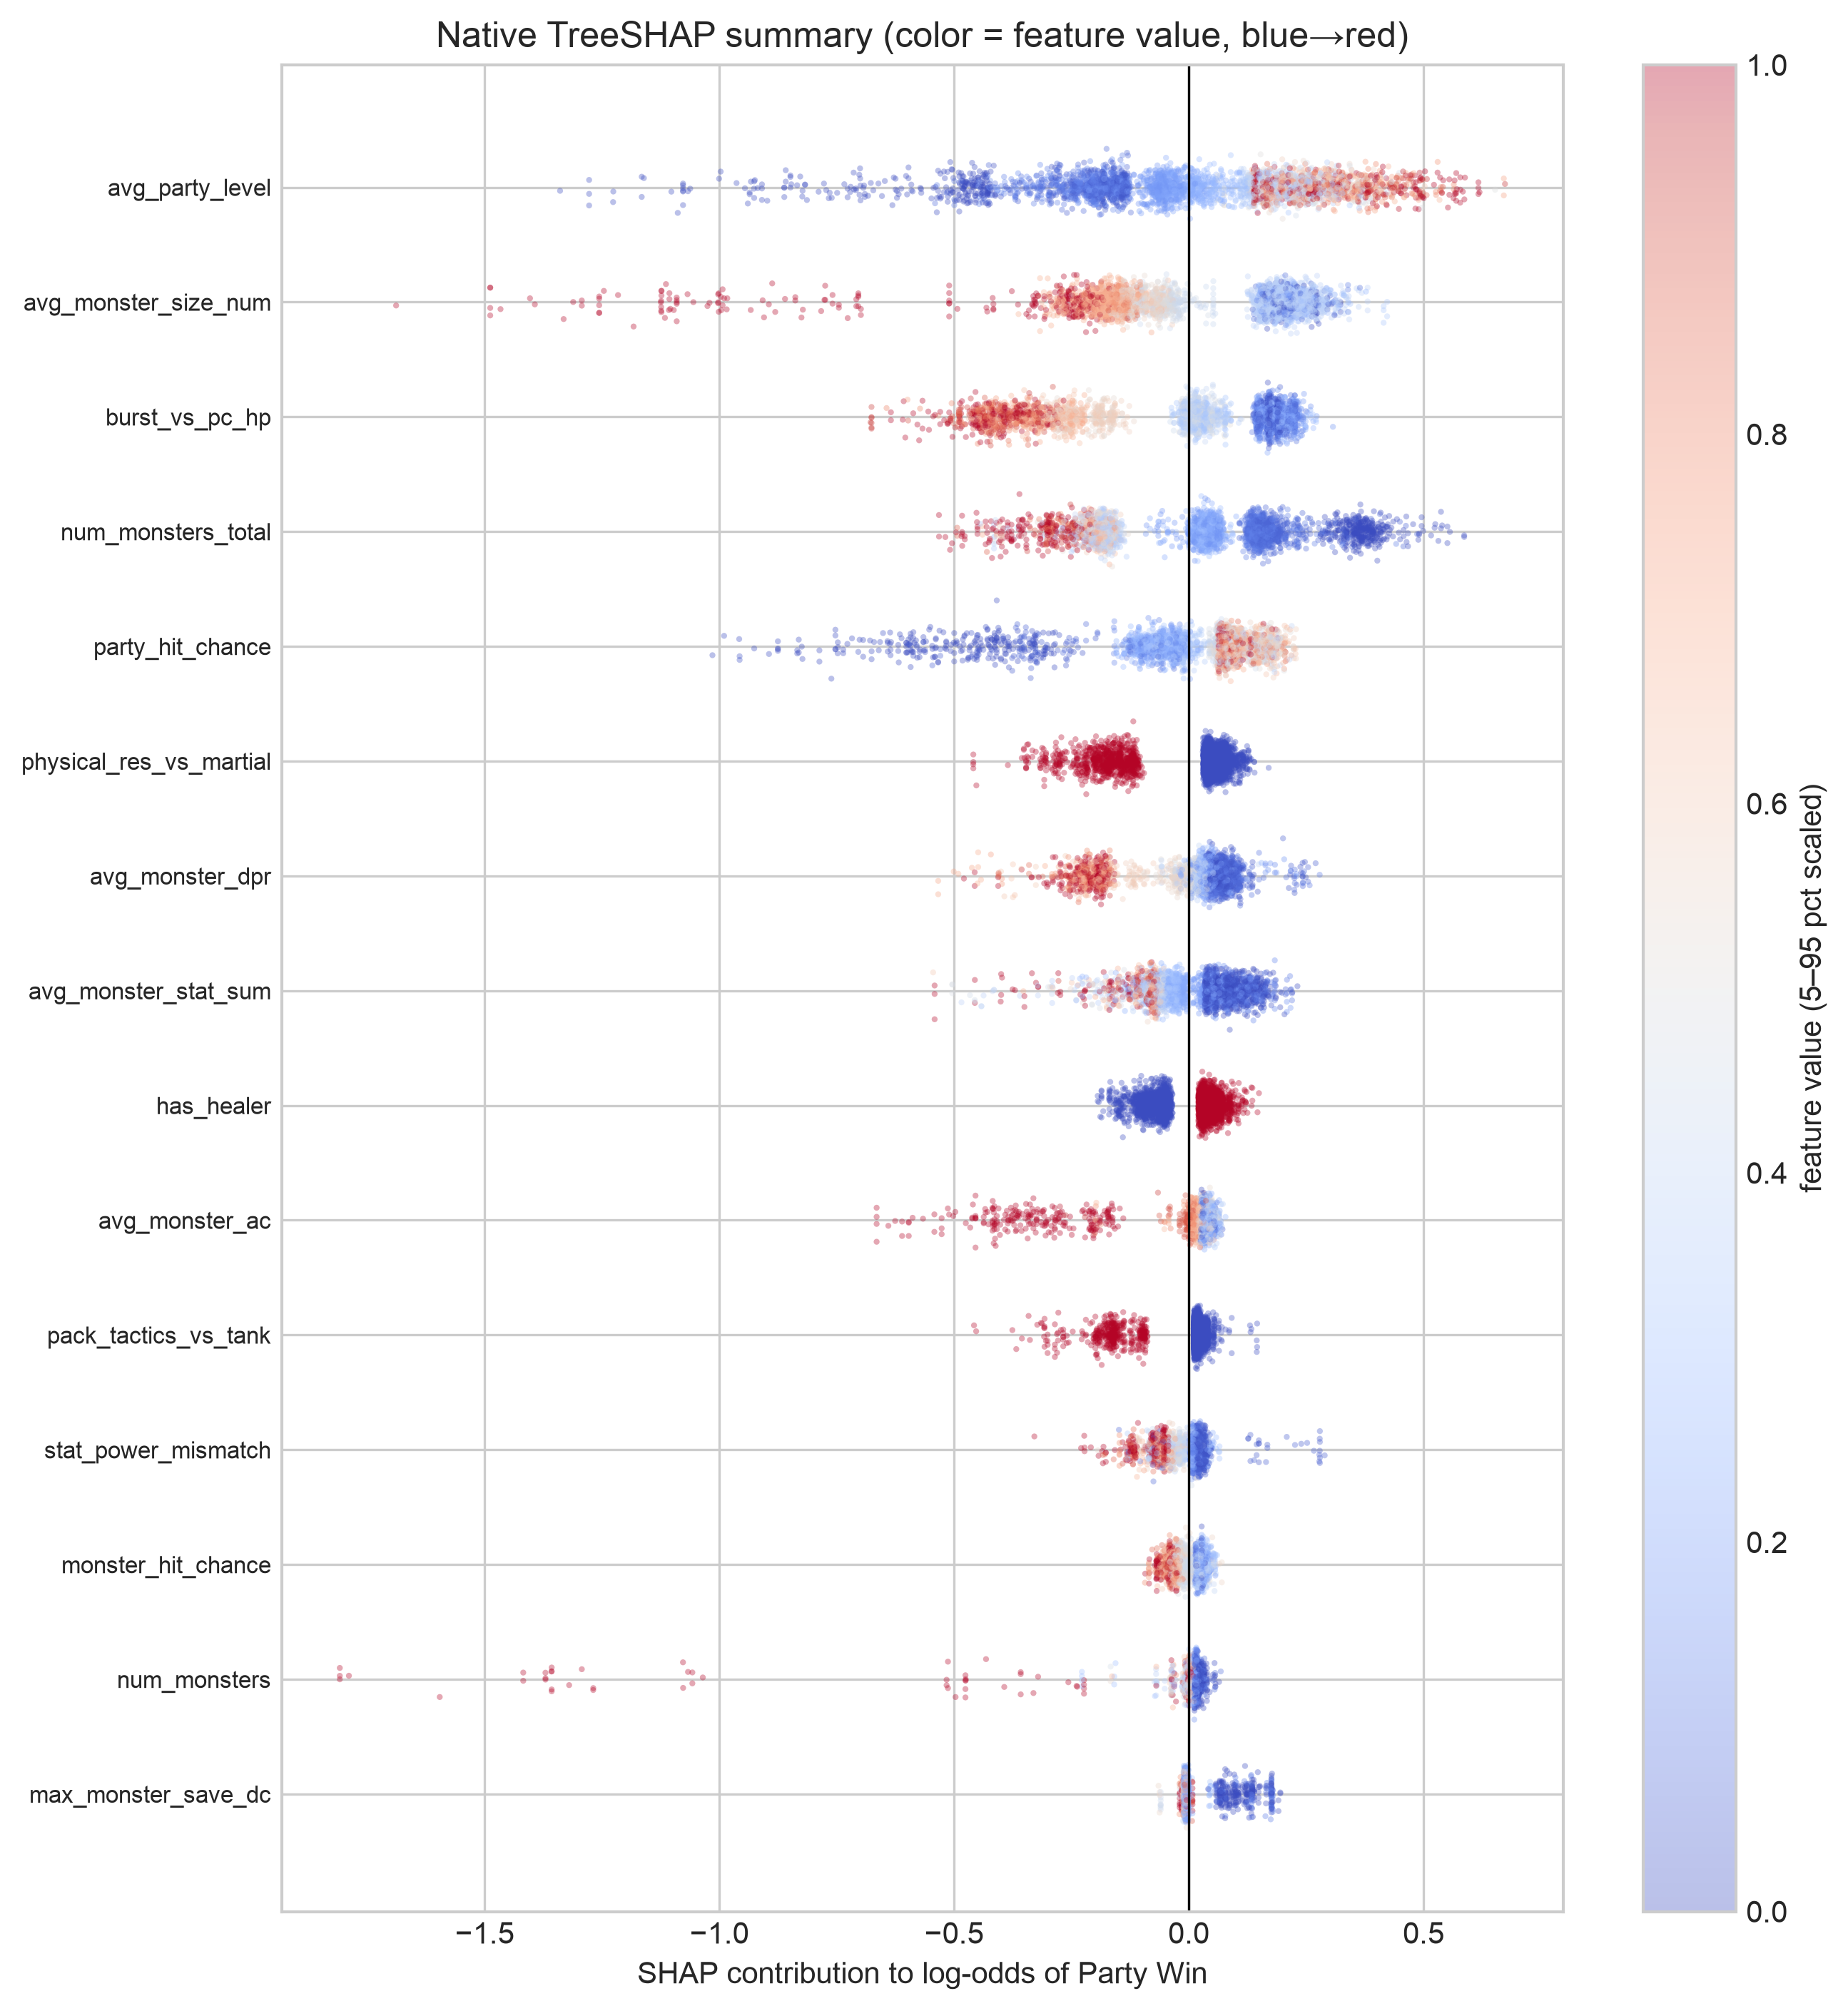
\includegraphics[width=\textwidth]{shap_summary.png}\\
      \srcnote{TreeSHAP: level, size, burst-vs-HP, action economy lead}
  \end{columns}
\end{frame}

\begin{frame}{The model: gradient boosting with domain priors}
  \begin{columns}[T]
    \column{0.55\textwidth}
      \begin{itemize}
        \item \textbf{XGBoost}, 45 engineered features, tuned by Optuna (grouped-CV objective): 300 trees, depth 4, heavy subsampling — shallow and regularized, as noisy logs demand.
        \item \textbf{45 monotone constraints} = shape priors: higher party level can never hurt; more monster DPR can never help.
        \item Inputs clipped to legal 5e ranges $\Rightarrow$ graceful out-of-distribution behavior.
      \end{itemize}
    \column{0.43\textwidth}
      \begin{block}{Serving pipeline}
        \small FeatureEngineer $\to$ Imputer $\to$ XGBoost $\to$ \textbf{Platt calibration} — one pickle, feature math travels with the model.
      \end{block}
      \begin{exampleblock}{Why Platt, not isotonic}
        \small Isotonic's step function made 1 Lich $\equiv$ 2 Liches in the level search; sigmoid is smooth \emph{and} measured slightly better (Brier 0.1394 vs 0.1397).
      \end{exampleblock}
  \end{columns}
\end{frame}

\begin{frame}{Honest evaluation: the unit of leakage is the campaign}
  \begin{itemize}
    \item Encounters from one campaign share party, DM, house rules $\Rightarrow$ random splits leak.
    \item Everything is grouped by campaign: \textbf{StratifiedGroupKFold} CV, grouped holdout, and even the \textbf{calibration folds}.
    \item The gap between grouped CV (0.601) and naive splits \emph{is} the leakage, reported rather than hidden.
  \end{itemize}
  \begin{block}{Held-out campaigns ($n = 7{,}106$ encounters), bootstrap 95\% CIs}
    \centering
    \begin{tabular}{lcc}
      \toprule
      ROC-AUC & \textbf{0.657} & [0.638, 0.674] \\
      Brier score & \textbf{0.139} & [0.134, 0.145] \\
      PR-AUC & 0.874 & — \\
      \bottomrule
    \end{tabular}
  \end{block}
\end{frame}

\begin{frame}{Calibration: the product consumes probabilities}
  \begin{columns}[T]
    \column{0.5\textwidth}
      \begin{itemize}
        \item ``Which level gives 65\% wins?'' is meaningless if 65\% doesn't mean 65\%.
        \item On held-out campaigns the curve hugs the diagonal where the data mass lives (0.8–0.9), with mild overconfidence in the lowest bins.
        \item AUC $\approx 0.66$ is \textbf{honest, not weak}: the outcome is genuinely noisy (dice, tactics, unrecorded items) and the base rate is 83\%.
      \end{itemize}
    \column{0.47\textwidth}
      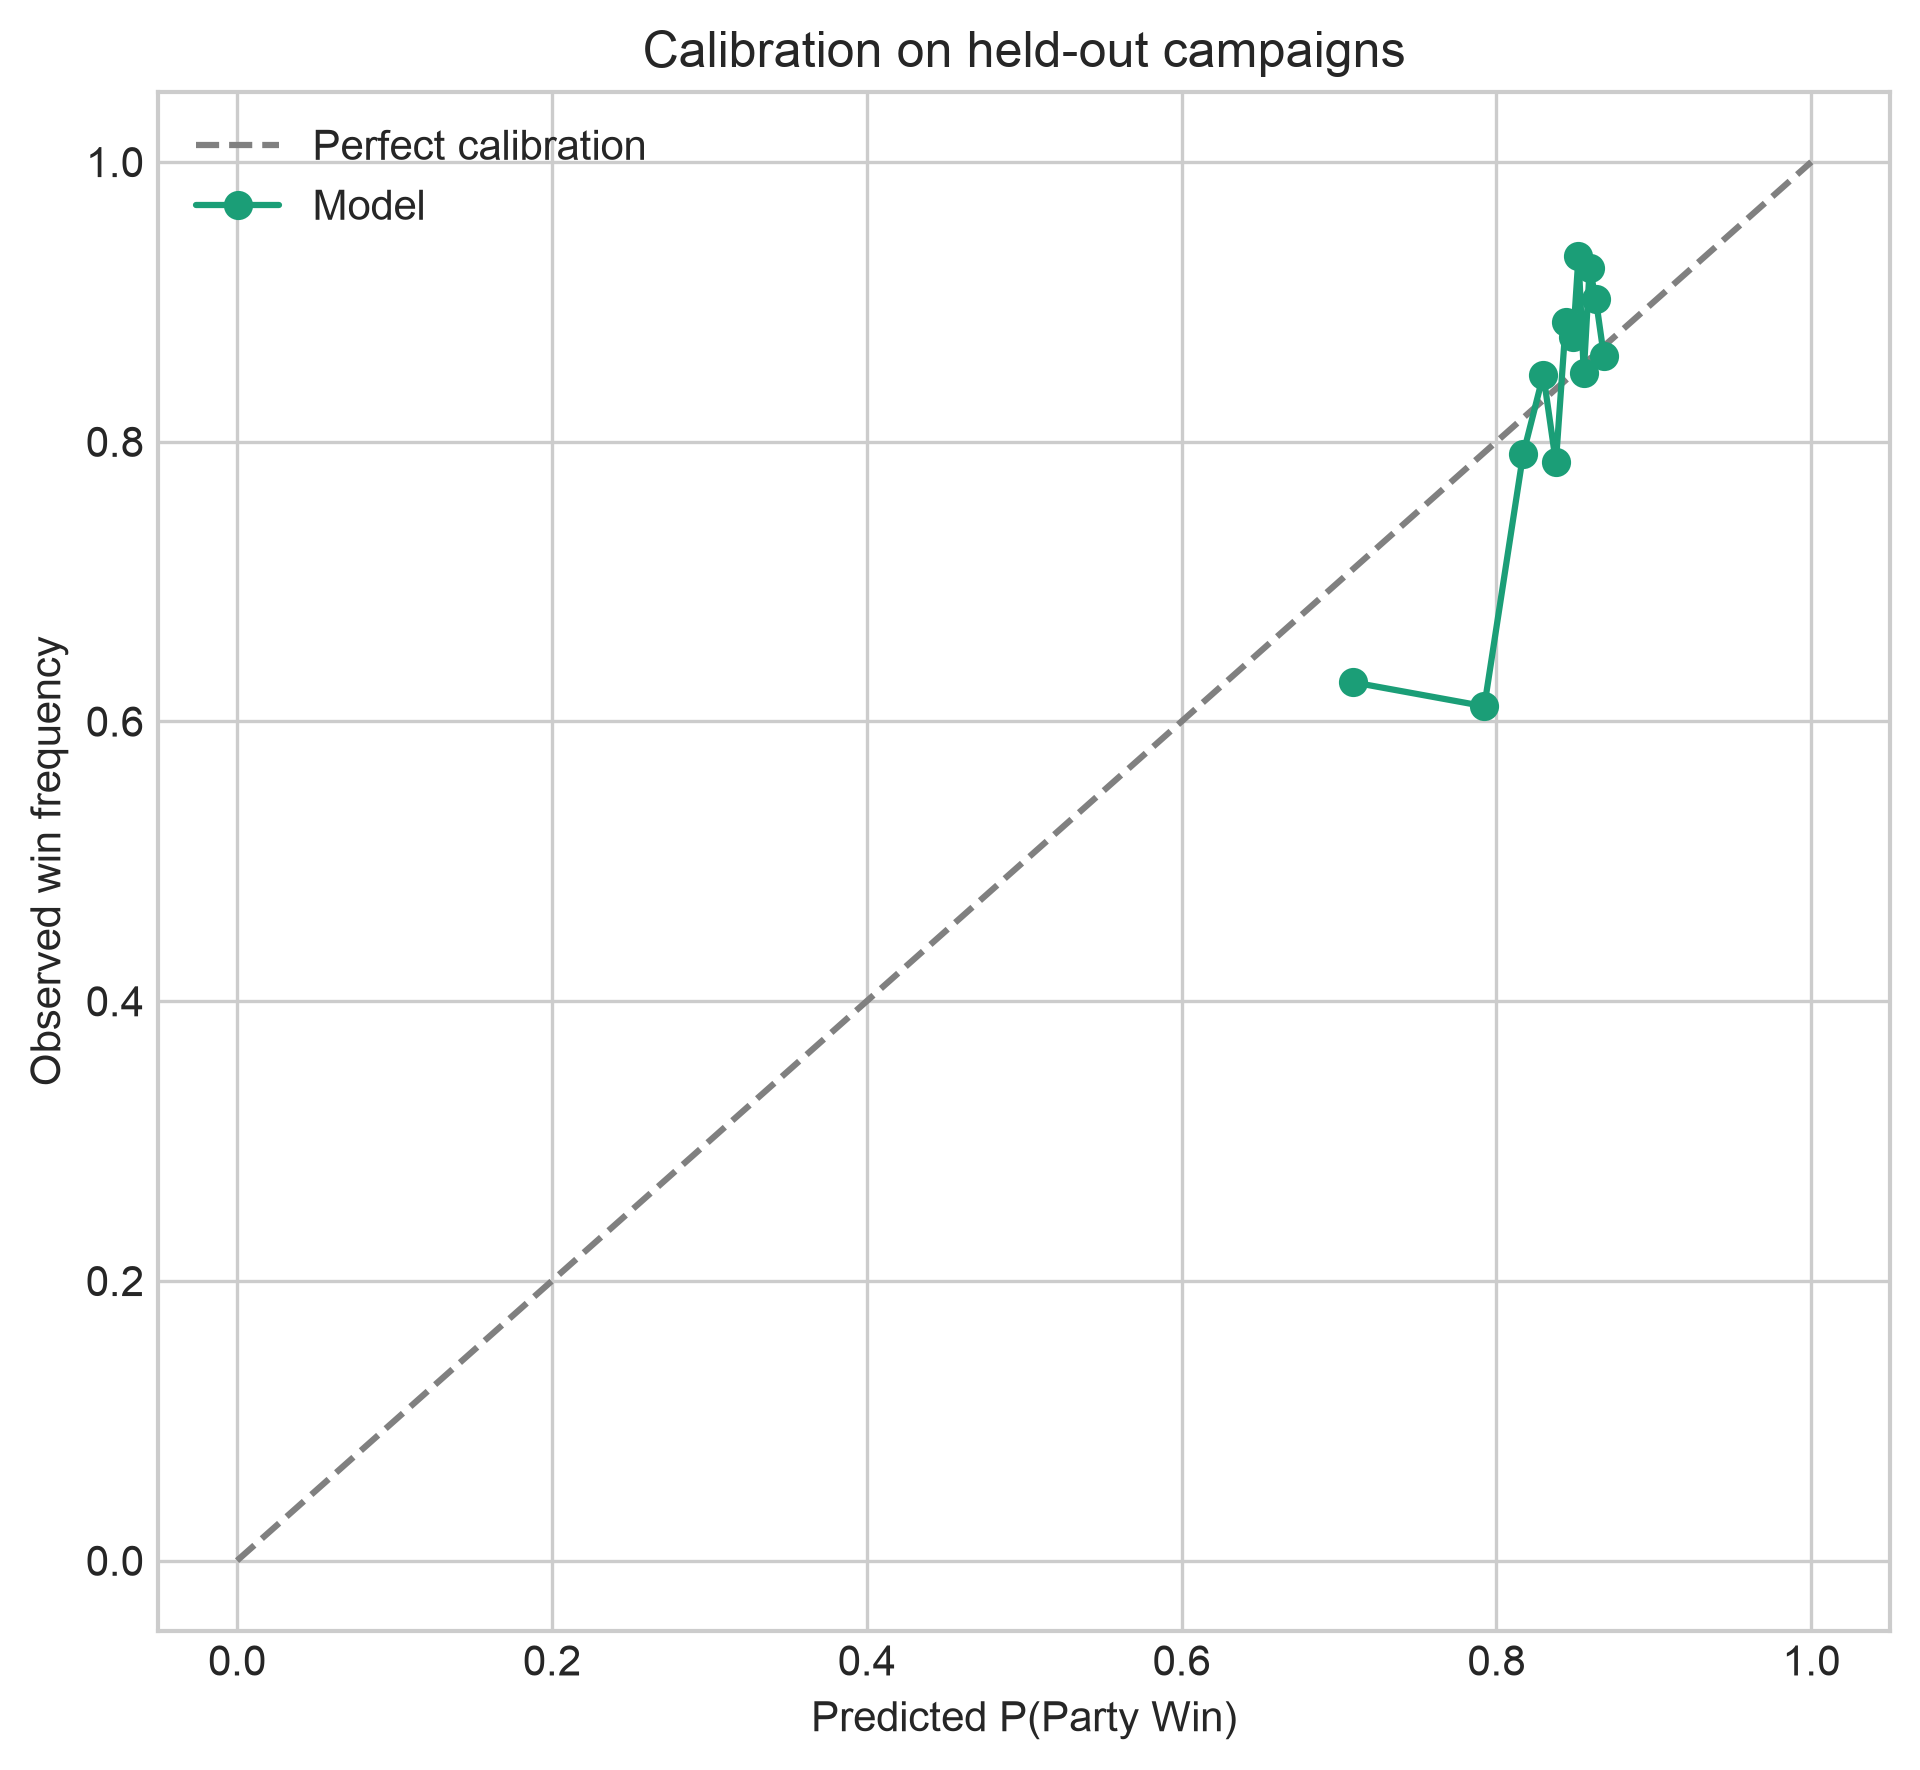
\includegraphics[width=\textwidth]{calibration_curve.png}
  \end{columns}
\end{frame}

\begin{frame}{A model that wins AUC and still loses}{The single most instructive result of the project}
  \begin{columns}[T]
    \column{0.5\textwidth}
      \small
      \begin{itemize}
        \item Ridge logistic \textbf{beats} XGBoost on observational risk: grouped-CV AUC \textbf{0.655 vs 0.614}.
        \item Promoted to production, it rated \alert{8 Liches as trivial} and a 10{,}000-HP monster as beatable.
        \item The coefficients show why: \texttt{num\_monsters}, \texttt{total\_dpr}, \texttt{burst} all \emph{positive}; \texttt{avg\_party\_level} \emph{negative} — selection confounding (harder content is served to stronger parties).
        \item[] \textbf{\textcolor{sapienzaRed}{Lesson: the app asks \emph{interventional} questions. Prediction $\neq$ decision.}}
      \end{itemize}
    \column{0.47\textwidth}
      \centering
      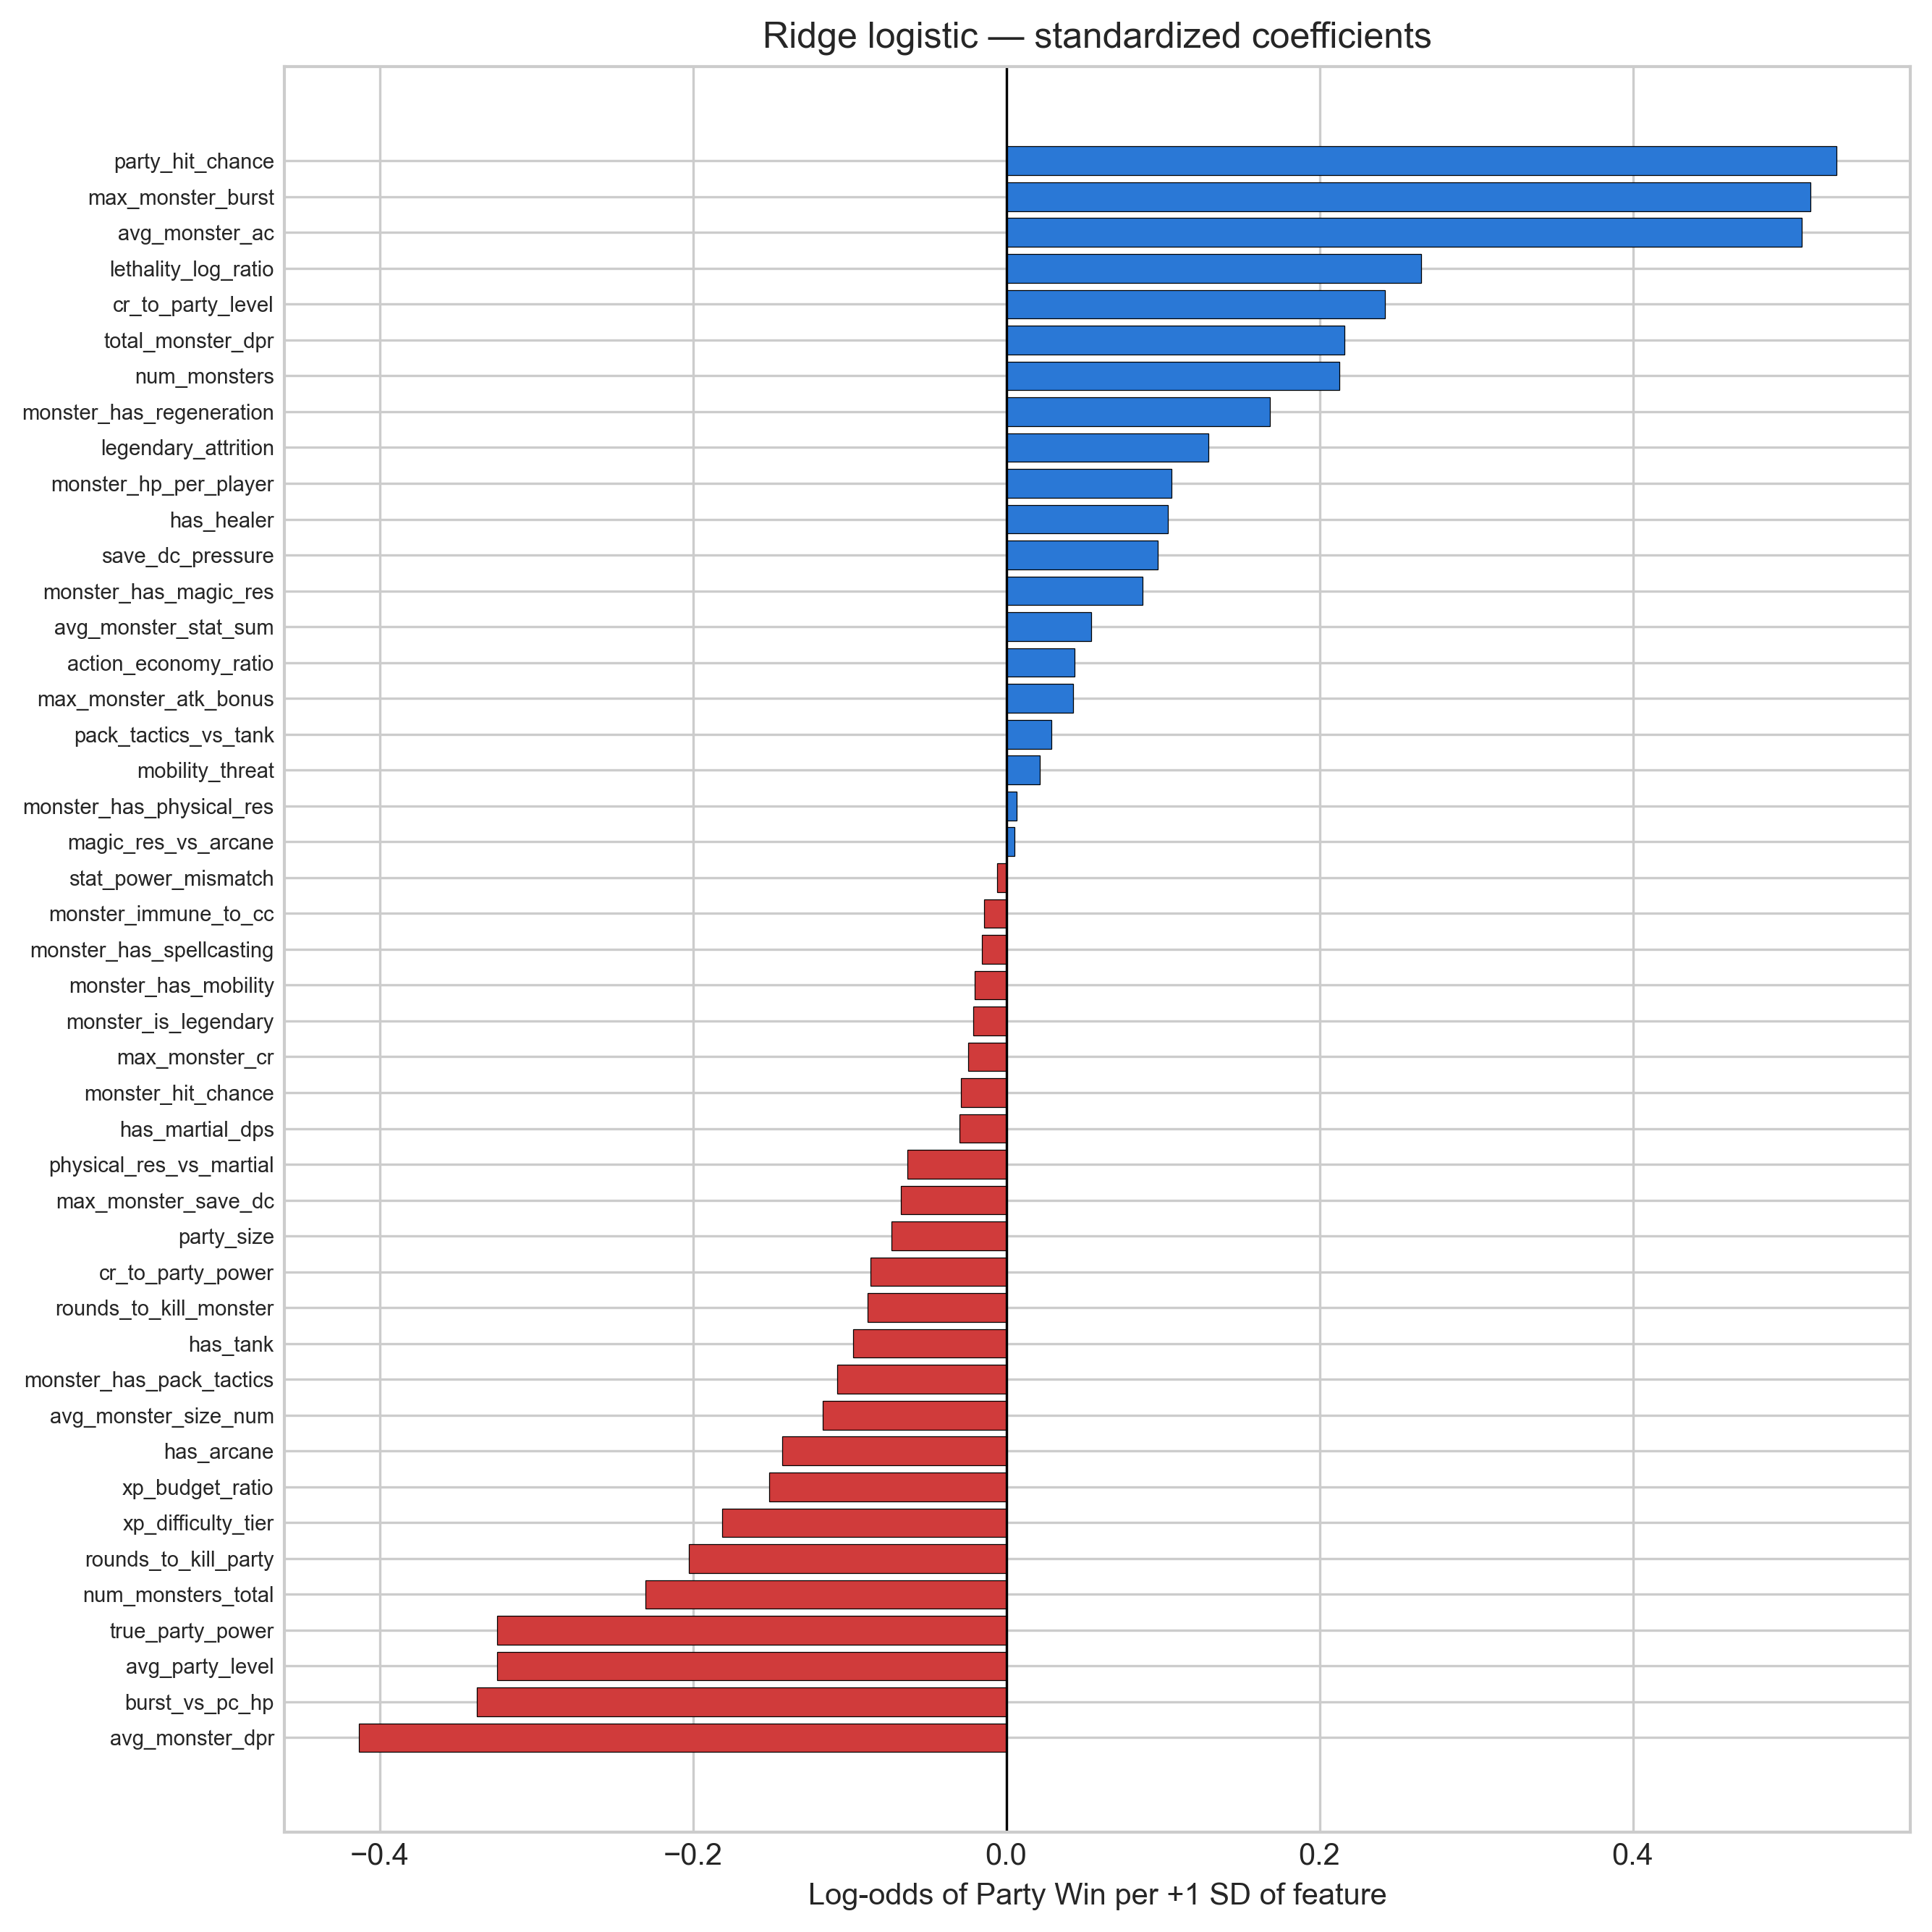
\includegraphics[height=0.74\textheight]{logistic_coefficients.png}
  \end{columns}
\end{frame}

% ════════════════════════════════════════════════════════════════════════════
\partdivider{3}{Where the data lies: guards \& simulation}{NOME 3}
\section{Part 3 — Guards \& simulation}

\begin{frame}{The bug that started it: 19 Liches, ``level 8''}
  \begin{itemize}
    \item Early model: 19 CR-21 Liches $\to$ beatable by a level-8 party at 66\%.
    \item Root cause is in the \emph{data}, not the code: fights the damage math calls hopeless (party deleted in $\leq 1$ round) were still ``won'' \textbf{84.5\%} of the time at real tables.
    \item \textbf{DM mercy}: fudged rolls, retreats recorded as wins, reinforcements. The logs answer ``what happens at tables'' — the app asks ``what if you fought \emph{to the death}''.
  \end{itemize}
  \begin{block}{Estimand mismatch}
    No amount of training data fixes this: the counterfactual question is simply not in the observational distribution. This motivates \emph{explicit domain guards}.
  \end{block}
\end{frame}

\begin{frame}{Three guards between the model and the user}
  \begin{enumerate}
    \item \textbf{Shape priors + clipping} — monotone constraints and legal-range clipping: absurd homebrew degrades gracefully.
    \item \textbf{Roster dominance} — count-weighted averages dilute (Lich + 6 goblins ``looks easier'' than the Lich alone); we score every homogeneous sub-roster and take the \textbf{minimum} win probability: adding monsters can never help the party.
    \item \textbf{Deathmatch physics cap} — $P(\text{win}) \leq \min(\sigma(A\,s - C\ln k + B),\ \Lambda)$: $s$ = rounds the party survives, $k$ = rounds to kill the roster, $\Lambda$ = interpolated simulator lattice. Originally hand-tuned\ldots
  \end{enumerate}
  \begin{exampleblock}{}
    \centering \ldots and hand-tuned constants are a weakness — so we calibrated them externally.
  \end{exampleblock}
\end{frame}

\begin{frame}{Battlecast: simulated deathmatches as external ground truth}
  \begin{columns}[T]
    \column{0.55\textwidth}
      \begin{itemize}
        \item Battlecast = Monte Carlo 5e combat simulator (initiative, movement, spell slots, conditions) — \textbf{no DM mercy}, scripted optimal play.
        \item Engine vendored from the site's public assets $\to$ fully local \& reproducible; zero load on the service; full provenance file.
        \item One run = 2{,}000 trials $\Rightarrow$ a nearly noise-free \textbf{soft label} (SE $\leq$ 0.011).
      \end{itemize}
    \column{0.43\textwidth}
      \begin{block}{Designed grids — 304 cells, 490{,}640 battles}
        \small \textbf{guard} 180: CR \{2,5,10,15,21\} $\times$ count \{1..19\} $\times$ level \{1..20\}\\
        \textbf{mercy} 100: 25 SRD monsters $\times$ 4 levels\\
        \textbf{OOD} 24: HP$\times$\{1,5,20\}, AC+\{0,8\} clones
      \end{block}
      \srcnote{make battlecast — party fixed: Fighter+Cleric+Wizard+Rogue}
  \end{columns}
\end{frame}

\begin{frame}{Result 1: the guard, calibrated}
  \begin{columns}[T]
    \column{0.47\textwidth}
      \small
      \begin{itemize}
        \item Race fit on guard+OOD cells: $\sigma(\textbf{0.19}\,s - \textbf{2.09}\ln k + \textbf{4.12})$. Survival-only guards were blind to \textbf{attrition}: 1 Lich vs level 5 survives 4+ rounds $\to$ old cap 0.95, simulator \textbf{0.000}.
        \item TTK features can't price spell rotations $\to$ $\Lambda$ = monotone lattice over the boss grid: on grid cells served $=$ simulated.
        \item Lich ladder now: 1$\to$\textbf{11}, 2$\to$\textbf{16.5}, \textbf{3+ $\to$ beyond deadly} — the simulator's own 65\% crossings.
      \end{itemize}
    \column{0.5\textwidth}
      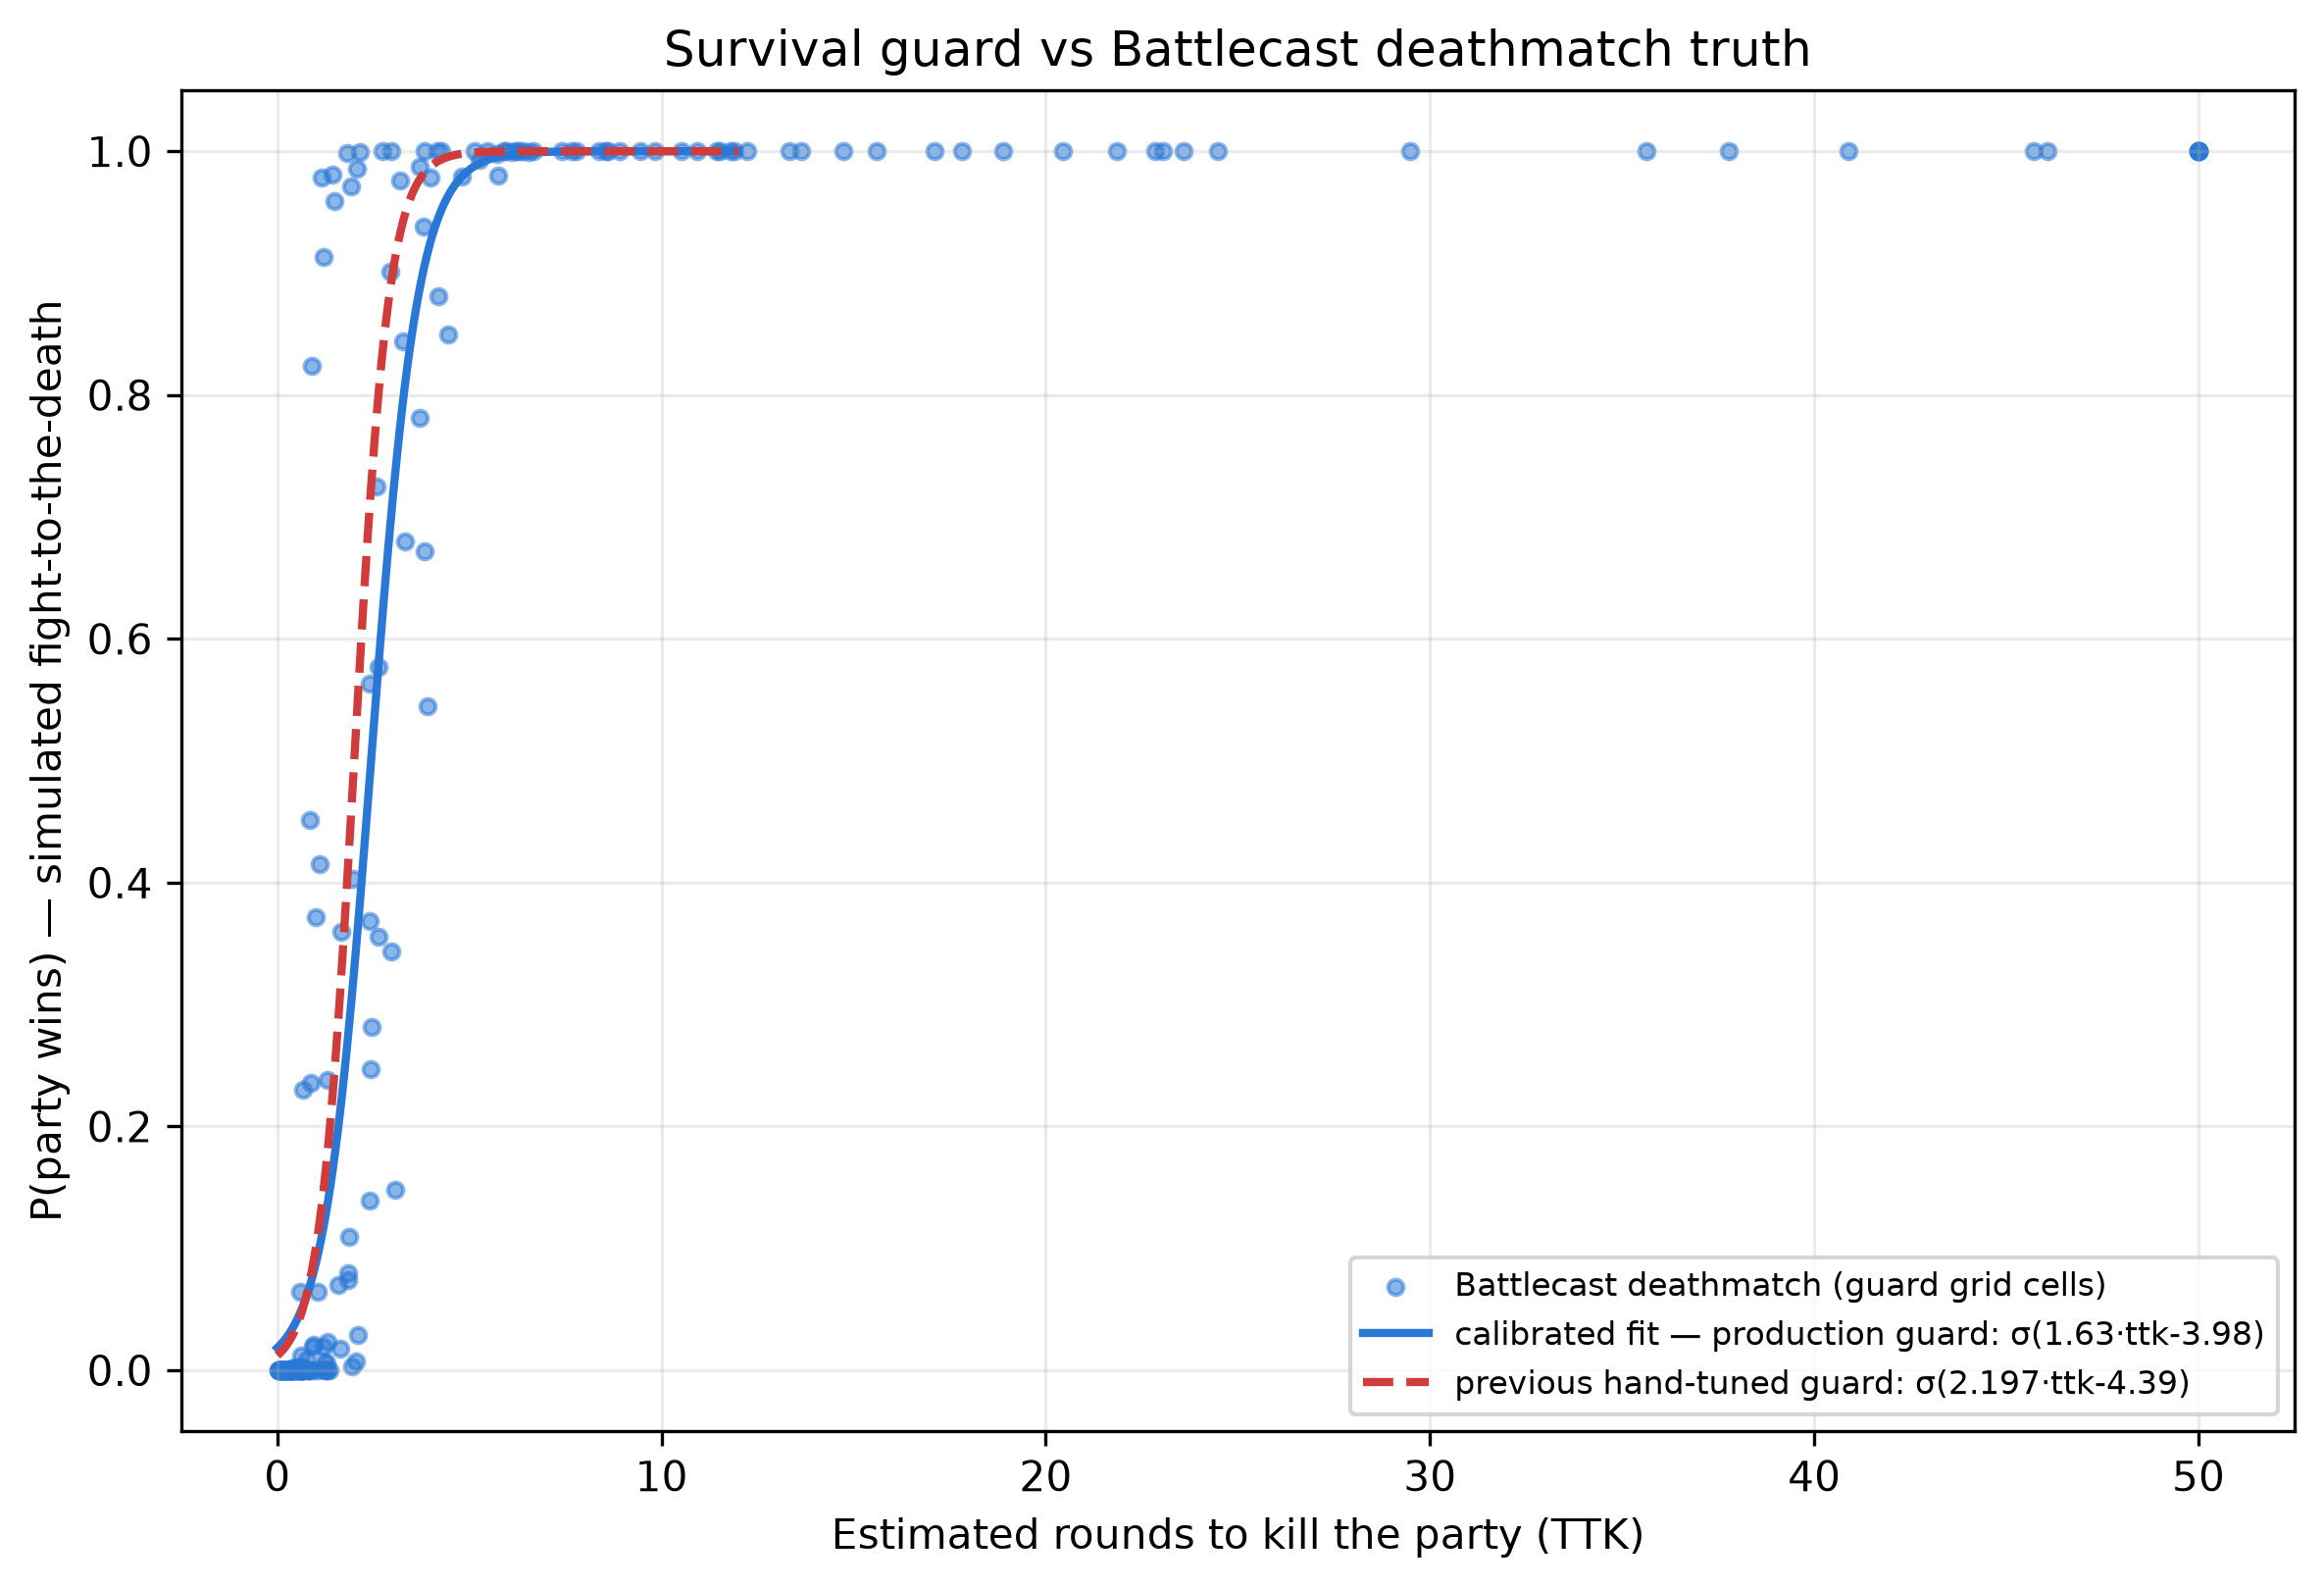
\includegraphics[width=\textwidth]{battlecast_guard_fit.png}
  \end{columns}
\end{frame}

\begin{frame}{Result 2: DM mercy, quantified}
  \begin{columns}[T]
    \column{0.47\textwidth}
      \small
      \begin{itemize}
        \item Same encounters through both lenses: our model (table reality) vs Battlecast (deathmatch). Correlation \textbf{0.842}.
        \item The gap \textbf{crosses over}: $\approx$ \textbf{+0.28 above} sim on hard fights (mercy inflation), $\approx$ \textbf{$-$0.14 below} on easy ones (the 83\% ceiling).
        \item Real curated encounters are overwhelmingly deathmatch-easy — table danger is attrition, not hopeless matchups.
      \end{itemize}
      \srcnote{Few hard-fight cells: +0.28 is directional. OOD: extremes agree (HP$\times$20 $\to$ $P\approx0$), mid ranking moderate (Spearman 0.54).}
    \column{0.5\textwidth}
      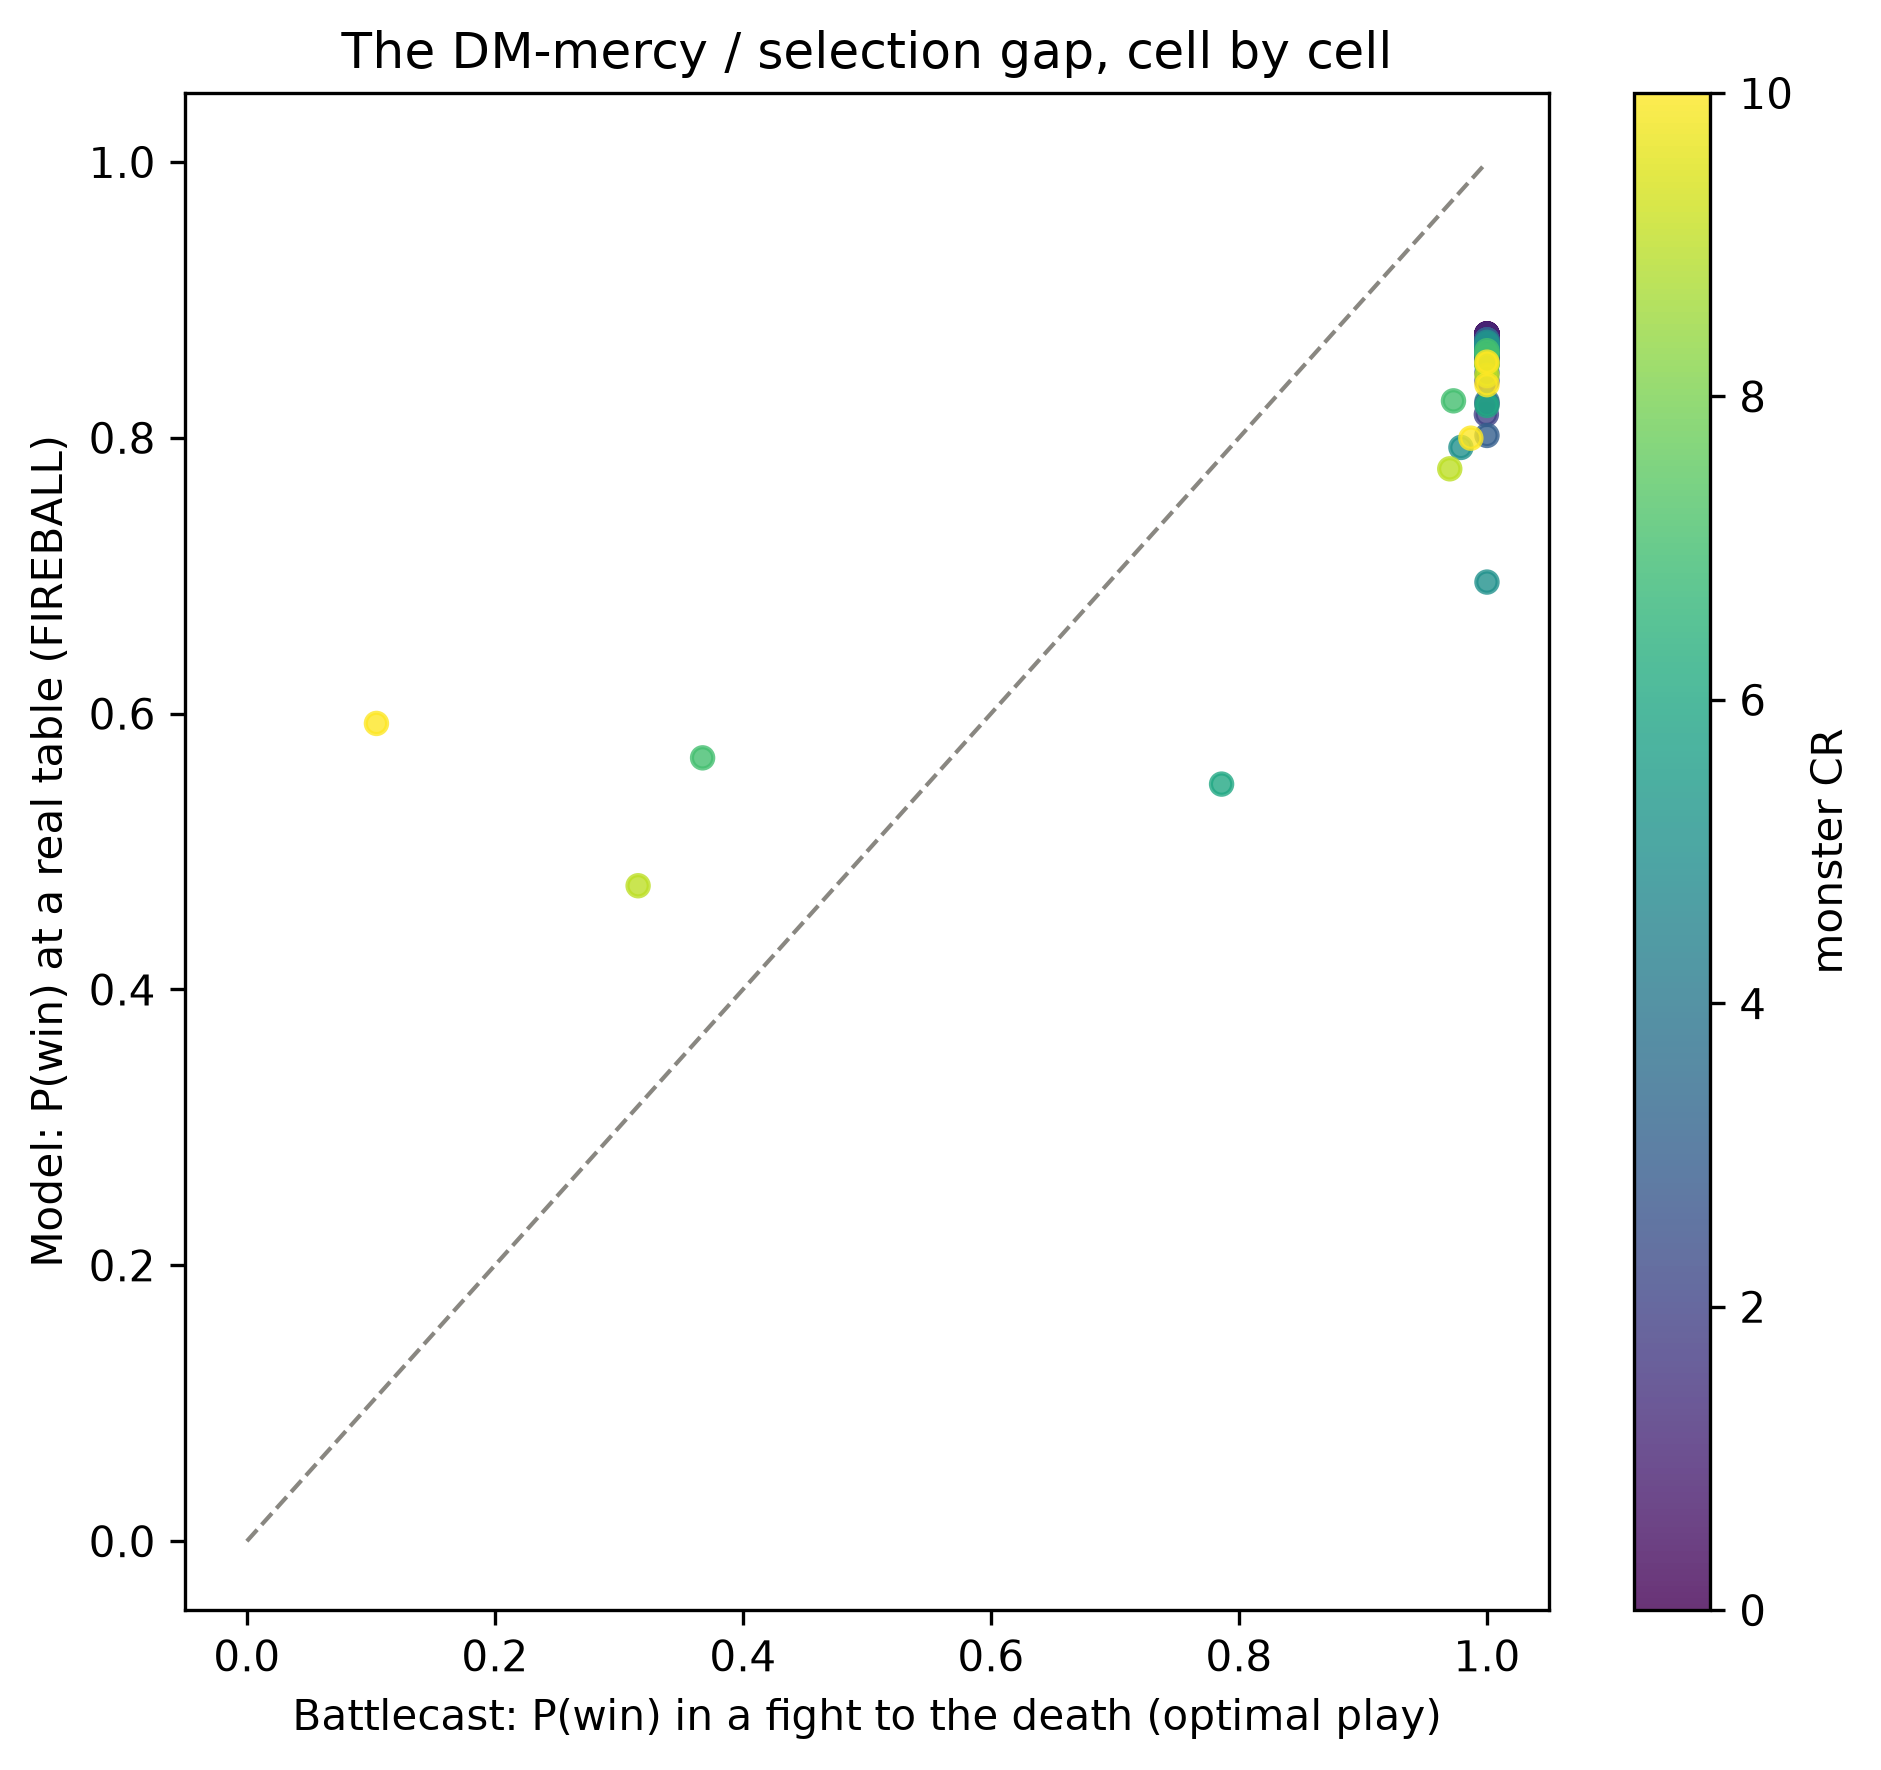
\includegraphics[width=\textwidth]{battlecast_mercy_gap.png}
  \end{columns}
\end{frame}

% ════════════════════════════════════════════════════════════════════════════
\partdivider{4}{Benchmarks, the product \& what we learned}{NOME 4}
\section{Part 4 — Benchmarks \& product}

\begin{frame}{The course toolbox, applied where each tool fits}
  \begin{columns}[T]
    \column{0.52\textwidth}
      \begin{itemize}
        \item \textbf{Model zoo under identical grouped CV}: ridge logistic 0.655, RFF kernel logistic 0.624, XGBoost 0.614 (AUC).
        \item \textbf{Kernel two-sample test (MMD)}: train vs held-out campaign features — MMD$^2 = 0.00031$, permutation $p = 0.12$: \emph{no covariate shift}; the CV-holdout gap is outcome variance, validating the split design.
        \item \textbf{Gaussian Process} CR predictor ($n=797$ monsters): MAE \textbf{0.86} vs XGBoost 0.94, $R^2$ 0.954 — and 95\% predictive intervals with \textbf{0.95 empirical coverage}.
      \end{itemize}
    \column{0.45\textwidth}
      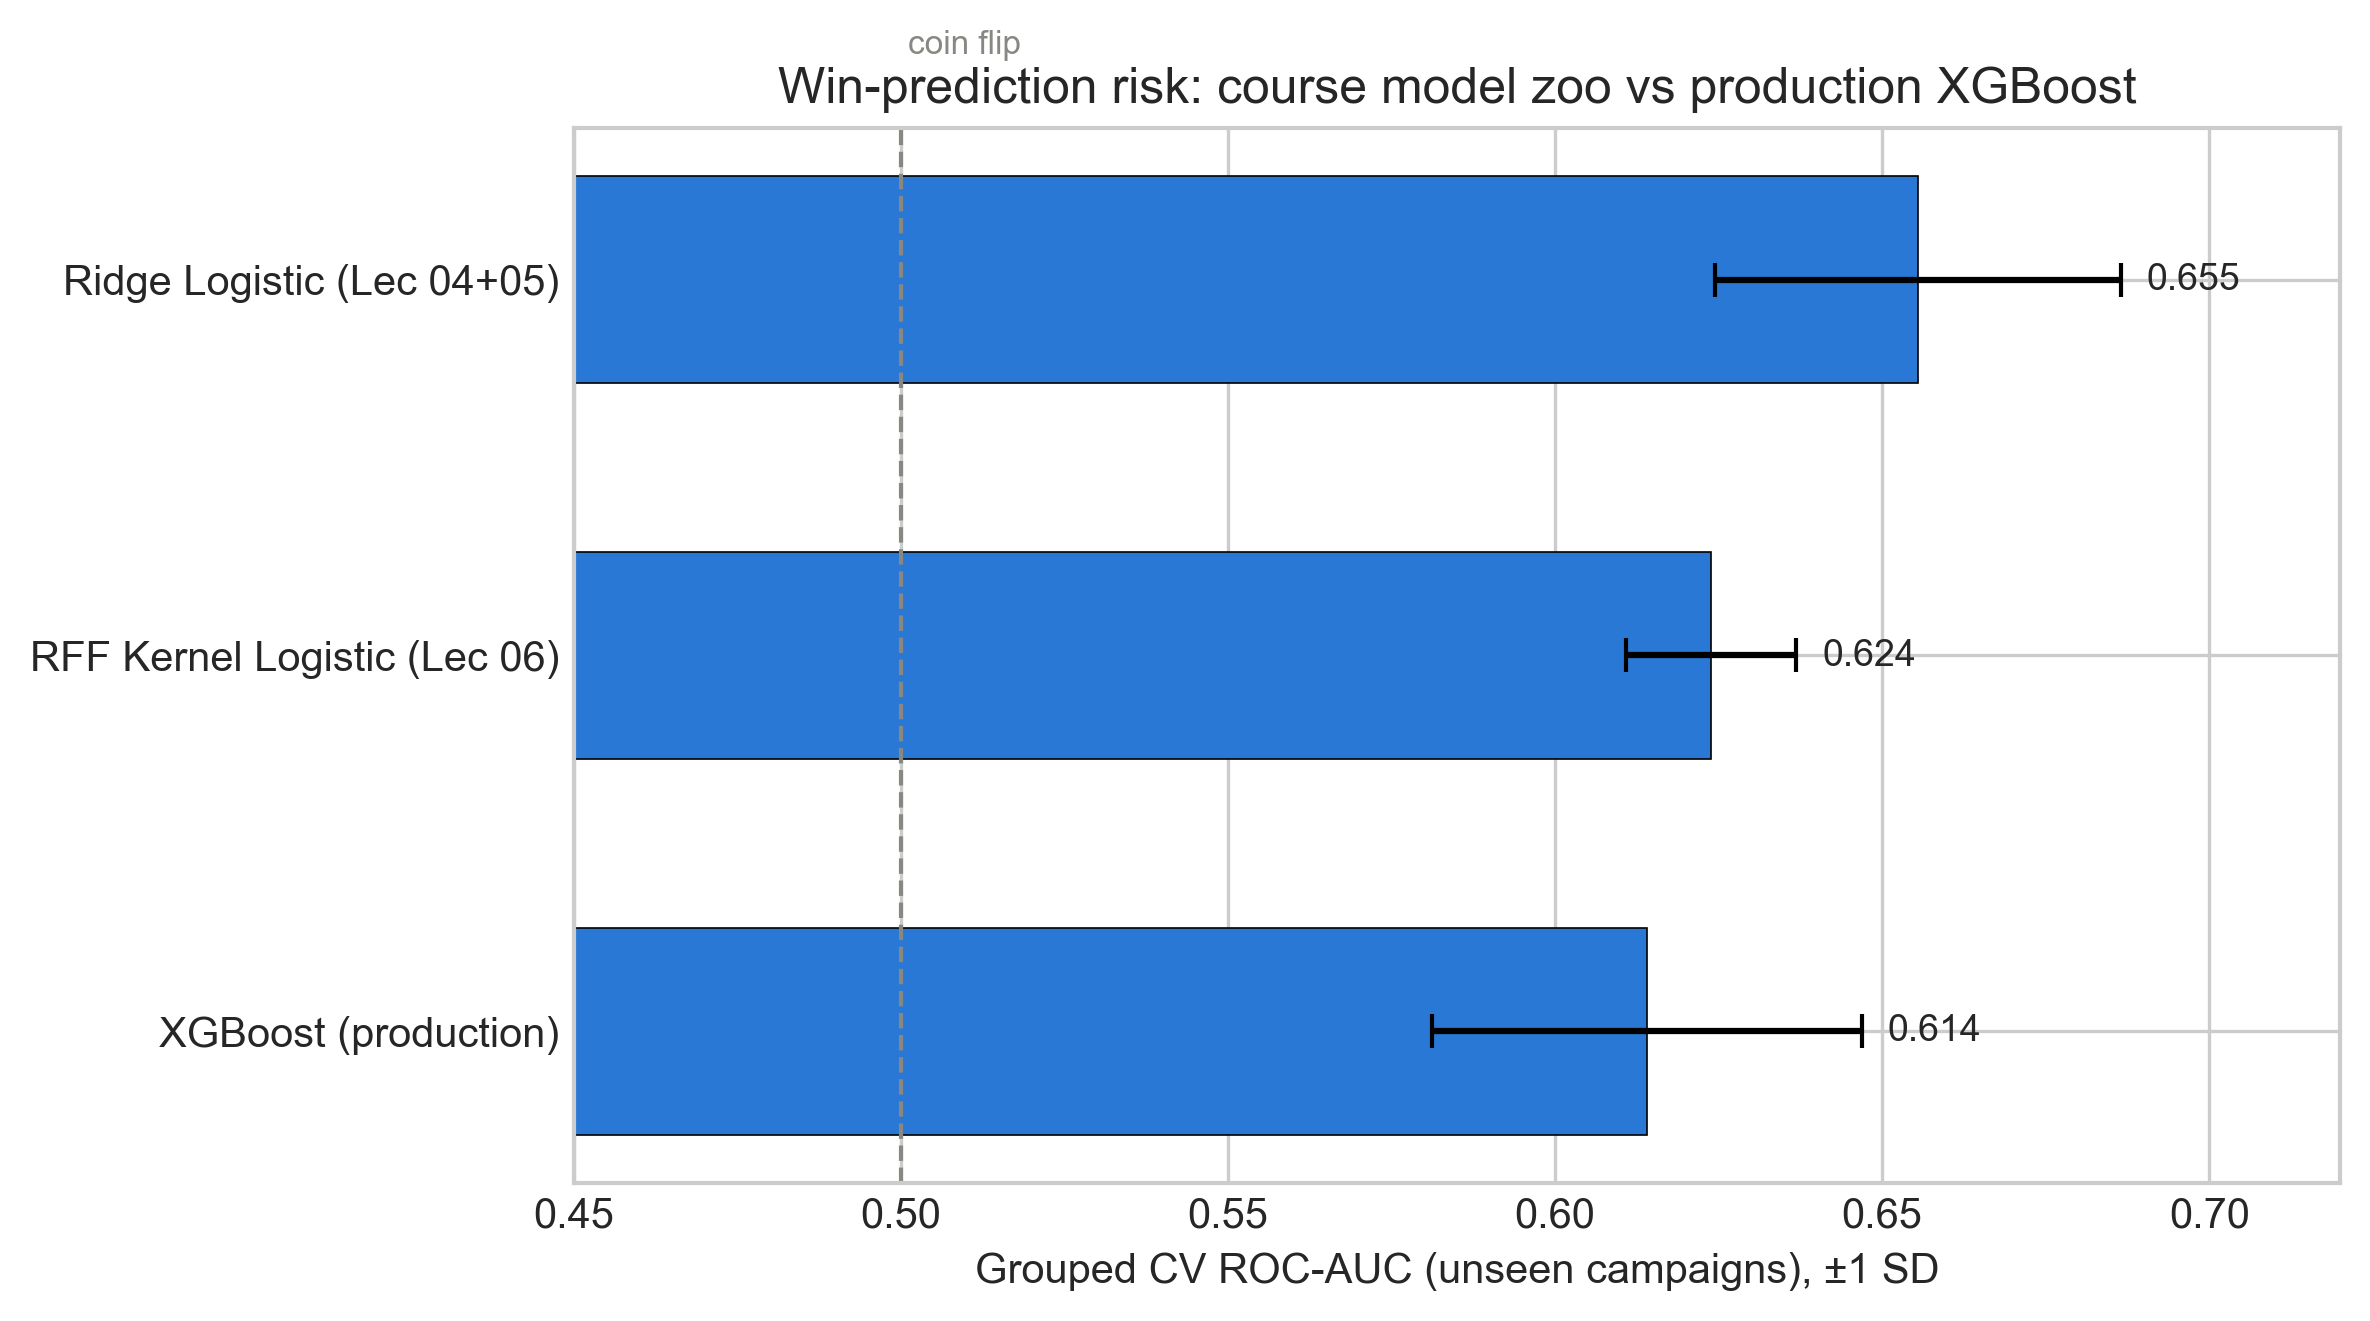
\includegraphics[width=\textwidth]{model_comparison.png}
      \srcnote{RFF = Rahimi–Recht random features: the Lec-06 kernel machine at $n \approx 28$k}
  \end{columns}
\end{frame}

\begin{frame}{One more ablation: synthetic balancing hurts}
  \begin{itemize}
    \item CTGAN-generated synthetic losses (leakage-guarded: fitted on training campaigns only) to ``balance'' the 83/17 classes.
    \item Same holdout, same pipeline: real data \textbf{AUC 0.657 / Brier 0.139} vs GAN-balanced \textbf{0.638 / 0.186}.
    \item Balancing shifts the predicted base rate to 0.61 — it \emph{destroys calibration} to fix a problem proper scoring rules never had.
  \end{itemize}
  \begin{block}{Takeaway}
    With a proper loss and calibration, class imbalance is a non-problem; resampling ``fixes'' cost more than they buy.
  \end{block}
\end{frame}

\begin{frame}{The product: a live encounter appraiser}
  \begin{columns}[T]
    \column{0.55\textwidth}
      \begin{itemize}
        \item \textbf{Streamlit app}: official-bestiary lookup, homebrew appraiser, mixed-monster encounter builder.
        \item Shows both verdicts side by side: \emph{by-the-book} (real DMG math) vs \emph{True Lethality Level}, with win-probability curves per party composition and a size$\times$level heatmap.
        \item Target win rate is a user slider — ``fair'' is a policy, not a constant.
      \end{itemize}
    \column{0.42\textwidth}
      \begin{block}{Try it}
        \centering\texttt{dnd-appraising.streamlit.app}
      \end{block}
      \begin{exampleblock}{Engineering rigor}
        \small 64 unit tests + 13 behavioral axioms (\texttt{make verify}); bootstrap CIs; append-only experiment log; pinned environment; one-command pipeline (\texttt{make retrain}).
      \end{exampleblock}
  \end{columns}
\end{frame}

\begin{frame}{Limits — stated, not hidden}
  \begin{itemize}
    \item \textbf{Observational ceiling}: AUC $\approx$ 0.66 on a noisy, 83\%-win world; the model ranks encounters well but is no oracle.
    \item \textbf{Estimand mismatch} handled by an explicit, now sim-calibrated guard — a modeling \emph{choice}, documented and tested, not learned end-to-end.
    \item \textbf{Simulator caveats}: 2024-SRD ruleset vs 2014-era logs; scripted optimal play $\Rightarrow$ deathmatch results are an upper bound.
    \item Thin support where it matters most (hard fights): future work = VTT instrumentation, post-encounter forms with explicit retreat/fudge labels, an all-SRD replay grid.
  \end{itemize}
\end{frame}

\begin{frame}{Five takeaways}
  \begin{enumerate}
    \item \textbf{Validate by the unit of leakage} (campaigns) — or every number is fiction.
    \item \textbf{Calibrate} when the product consumes probabilities; measure it (Brier, curves), don't assume it.
    \item \textbf{Prediction $\neq$ decision}: a better-AUC model can be unusable; constraints encode the difference.
    \item \textbf{Know your estimand}: observational data can't answer counterfactual questions — simulation can, and can even calibrate your priors.
    \item \textbf{The rulebook deserved a fair trial} — and honestly implemented, it still loses to 34{,}907 real fights.
  \end{enumerate}
\end{frame}

{\setbeamercolor{background canvas}{bg=sapienzaRed}
\begin{frame}[plain]
  \vfill\centering
  {\color{white}\Huge\bfseries Grazie!\\[2ex]}
  {\color{white}\large Questions welcome — or bring us a monster to appraise.\\[3ex]}
  {\color{white!80!sapienzaRed}\small \texttt{dnd-appraising.streamlit.app}\quad·\quad\texttt{github.com/danpinocontrollino/project-dnd}}
  \vfill
\end{frame}}

\end{document}
